%% example.tex
%% Jeremy Singer
%% 16 Oct 12

\documentclass{mpaper}

\usepackage[caption=false]{subfig}

\begin{document}

\title{QUICsilver: Optimising QUIC for use with Real-Time Multimedia Traffic}
\author{Vivian Band}
\matricnum{2038561}

\maketitle

\begin{abstract}
  % Four sentences:
  %  - State the problem
  QUIC, a fully reliable stream-oriented transport protocol, is gaining popularity but is too high-latency to use as a transport for real-time multimedia playback.
  
  %  - Say why it's an interesting problem
    As a userspace protocol, QUIC can be easily modified due to not requiring kernel modifications. The retransmission behaviours can be altered to be partially reliable rather than fully reliable.
  
  %  - Say what your solution achieves
  QUICsilver, the partially reliable QUIC implementation developed in this project, performs selective retransmissions based on deadline awareness to increase the throughput of useful data while avoiding stalls to keep latency low.
  
  %  - Say what follows from your solution
  This solution shows that QUIC can be modified within a relatively short timeframe to better support real-time multimedia applications which have strict latency bounds.
  

\end{abstract}

%==================================================================================================
\section{Introduction}

% A good paper introduction is fairly formulaic. If you follow a simple set
% of rules, you can write a very good introduction. The following outline can
% be varied. For example, you can use two paragraphs instead of one, or you
% can place more emphasis on one aspect of the intro than another. But in all
% cases, all of the points below need to be covered in an introduction, and
% in most papers, you don't need to cover anything more in an introduction.
%
% Paragraph 1: Motivation. At a high level, what is the problem area you
% are working in and why is it important? It is important to set the larger
% context here. Why is the problem of interest and importance to the larger
% community?
According to \textit{The Zettabyte Era} white paper by Cisco \cite{CISCO2015}, the percentage of Internet Protocol (IP)\cite{IP-RFC} traffic carrying multimedia data will increase from 73\% of all IP traffic in 2016 to 83\% by 2021. Live video and online gaming are commonly used applications on the modern Internet and are predicted to form 13\% and 4\% of all IP traffic by 2021 respectively; these applications have strict latency bounds in order to appear to respond in real-time to user input.

QUIC is a modern, fully-reliable userspace transport protocol which is being adopted as an alternative to the Transmission Control Protocol (TCP)\cite{TCP-RFC} for delay-tolerant client-server applications. QUIC accounted for a over 30\% of Google's outbound traffic in 2016 \cite{Langley2017}, and traffic using QUIC as a transport protocol represented up to 9.1\% of global Internet traffic in 2018 \cite{Ruth2018}. However, standard QUIC not suitable for real-time applications due to high latencies caused by head-of-line blocking as a result of its reliability guarantees and in-order delivery of data to the application. QUIC is a userspace protocol which uses the Userspace Datagram Protocol (UDP) \cite{UDP-RFC} as a substrate, and can be modified more easily than kernel-level implementations of transport protocols such as TCP. The lack of required behaviours in UDP allows QUIC to be significantly modified, meaning that QUIC can be adapted for use with real-time multimedia applications.
  
  %  - Say why it's an interesting problem
Real-time multimedia applications typically use the Real-Time Transport Protocol (RTP) \cite{RTP-RFC}, an unreliable transport protocol which runs over UDP. This lack of retransmissions allows applications using UDP to maintain low latency, but modifying QUIC to be partially reliable in that it will perform selective retransmissions based on estimated playback deadlines has the potential to increase the throughput of useful data compared to a fully unreliable transport like RTP.

  %  - Say what your solution achieves
QUICsilver is a partially reliable implementation of QUIC which achieves low-latency by allowing some packet loss, subject to playback deadlines, in order to improve the throughput of data to the receiver application. Video playback quality can be further improved by taking advantage of existing retransmission behaviours in QUIC, allowing the retransmission of video frames which will still be useful when they reach the receiver as well as any dependent frames required for live ones. The RTP packets sent by QUICsilver are also protected by QUIC's Transport Layer Security version 1.3 (TLS 1.3) \cite{TLS-RFC} encryption mechanisms by default, offering extra privacy to users compared to standard RTP, as well as the potential for the parallel delivery of content through multiplexed content streams.
  
  %  - Say what follows from your solution
This paper shows that partial reliability eliminates the occurrence of stalls and cumulative playback delays encountered by standard, fully reliable QUIC by allowing a client to skip lost packets if the playback deadline is approaching for previously received packets with a higher packet number. This lack of stalling is observed for all loss rates; on low-latency links, QUICsilver maintains the strict latency bounds required for real-time applications even in challenging, high-loss environments.

The removal of items which will not be useful to the client based on predicted playback deadlines is important to avoid wasteful retransmissions, however, this results in I-frames and P-frames only being retransmitted on low-latency links: if 1 in every 10 frames sent is an I-frame, retransmissions of stale I-frames which have live dependent P-frames are only performed on links with a latency lower than 66.6ms. Beyond this, QUICsilver effectively functions as an unreliable transport with added security and in-built support for multiplexed content streams.


% Paragraph 2: What is the specific problem considered in this paper? This
% paragraph narrows down the topic area of the paper. In the first
% paragraph you have established general context and importance. Here you
% establish specific context and background.



% Paragraph 3: "In this paper, we show that...". This is the key paragraph
% in the introduction - you summarize, in one paragraph, what are the main
% contributions of your paper, given the context established in paragraphs 
% 1 and 2. What's the general approach taken? Why are the specific results
% significant? The story is not what you did, but rather:
%  - what you show, new ideas, new insights
%  - why interesting, important?
% State your contributions: these drive the entire paper.  Contributions
% should be refutable claims, not vague generic statements.

% Paragraph 4: What are the differences between your work, and what others
% have done? Keep this at a high level, as you can refer to future sections
% where specific details and differences will be given, but it is important
% for the reader to know what is new about this work compared to other work
% in the area.



% Paragraph 5: "We structure the remainder of this paper as follows." Give
% the reader a road-map for the rest of the paper. Try to avoid redundant
% phrasing, "In Section 2, In section 3, ..., In Section 4, ... ", etc.

The remainder of this paper is structured as follows. Section 2 explores the background knowledge of sending video content using RTP and section 3 reviews existing work on optimising reliable transport protocols for multimedia content. The design of QUICsilver is explained in section 4, and analysis of the tests performed to compare its performance to standard QUIC is conducted in section 5. Future work to improve QUICsilver is proposed in section 6, and conclusions about using QUIC for multimedia which have been gained from this project are discussed in section 7.

%==================================================================================================
% Concentrate single-mindedly on a narrative that:
%  - Describes the problem, and why it's interesting
%  - Describes your idea
%  - Defends your idea, showing how it solves the problem, and filling out
%    the details
% On the way, cite relevant work in passing, but defer discussion to the
% end.
%
% Introduce the problem, and your idea, using examples, and only then
% present the general case. Explain the idea as if your were speaking to
% someone using a whiteboard. Conveying the intuition is primary; details
% follow. Write in a top down manner: state broad themes and ideas first,
% then go into details.
%
% The introduction makes claims. The body of the paper provides evidence
% to support each claim. Check each claim in the introduction, identify
% the evidence, and forward-reference it from the claim. 
%==================================================================================================
\section{Background}

% The problem

\subsection{Video Frames} 
For multimedia applications, there are three types of video frames: intra-frames (I-frames), predicted frames (P-frames), and bidirectional predicted frames (B-frames). I-frames provide data for a whole image; the data required to specify this for most resolutions is in excess of the QUIC payload size of 1232 bytes, so a single I-frame must be sent using multiple QUIC packets (an I-frame is sent as 4 QUIC packets in this project). P-frames only describe changes in a small section of the display in relation to an I-frame; these are small enough to be transmitted in a single QUIC packet in their entirety, but the I-frame on which they depend must be noted to ensure the changes are applied to the correct base image. B-frames are even more compressed than P-frames due to referring to previous and next video frames to describe changes; B-frames are not included in this project due to time constraints and a focus on reducing transmission latencies rather than compression efficiencies.

\begin{figure}[h!]
 \centering
 \subfloat[An example of an I-frame, detailing an entire image]{
   
\includegraphics[scale=0.2]{images/bunny-i-frame}
   \label{bunny-i-frame}
 }
 \\
 \centering
 \subfloat[An example of a P-frame applied to an I-frame to change only the highlighted sections]{
   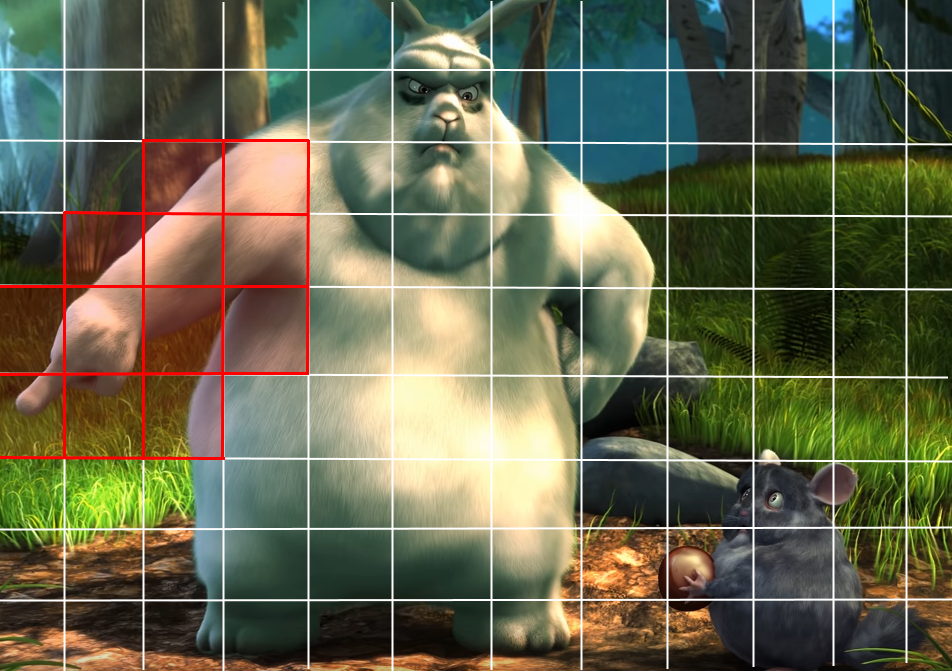
\includegraphics[scale=0.2]{images/bunny-p-frame}
   \label{bunny-i-frame}
 }
 \caption{Example of I-frames and P-frames}
 \label{frame-example}
\end{figure}

I-frames are sent to provide an initial image to work from and to refresh the image being played back to correct any glitches which may have occured as a result of P-frames being applied to an incorrect I-frame. P-frames are sent much more often, and make up the majority of sent video frames for live video streaming.


\subsection{Head-of-Line Blocking}

Reliable transports such as QUIC and TCP suffer from high latency due to head-of-line blocking. This occurs due to the guaranteed, ordered delivery of data: in order to ensure that all data is delivered in-order to an application, the protocol waits for missing packets to arrive before releasing data which was received previously in packets with a higher packet number.

\begin{figure}[h]
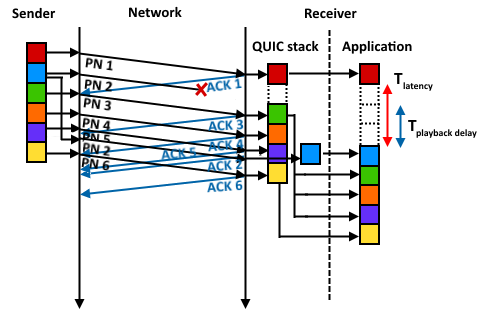
\includegraphics[scale=0.5]{images/head-of-line-blocking}
\centering
\caption{Head-of-line blocking in QUIC. The loss of packet number 3 prevents any subsequent packets being delivered to the application until it is received, causing the blue packet to have a stack latency of 1.5 times the round-trip time and a playback delay of 1 round-trip time.}
\label{hol}
\end{figure}

QUIC mitigates the impact of head-of-line blocking by using several streams demultiplexed 
over a single UDP socket. Although head-of-line blocking still occurs in response to loss, the 
obstruction is confined to a single stream rather than blocking the entire connection, as happens with TCP. However, this still causes unacceptably high latency for real-time media data being delivered on this stream: as illustrated in figure \ref{hol}, the total latency between the packet being sent the first time and finally being received by the application is 1.5 times the path's round-trip time. Allowing some loss under partial reliability is necessary to reduce stack to application latency.


%==================================================================================================
\section{Related Work}
QUIC-R, a set of real-time extensions to QUIC suggested by Perkins and Ott, contains valuable background information about the evolution of video streaming technologies and their potential place in QUIC. RTP was historically used to stream media on less reliable networks from the mid-1990s, but applications using this protocol are complex due to the mechanisms required to mitigate the effects of packet loss and out-of-order arrival. Dynamic Adaptive Streaming over HTTP (DASH) is less complex, providing media content in pre-encoded chunks through a series of HTTP \texttt{GET} requests; this approach has become more widely used as networks have increased in quality and demand has risen for unidirectional streaming (i.e. the content being sent is not impacted by the actions of the receiver and therefore has more relaxed latency bounds).


Adapting a mapping of RTP onto TCP specified in RFC 4751 \cite{RTP-TCP-RFC} for use with QUIC is discussed in the QUIC-R paper, but deemed unacceptable for applications with strict latency bounds. This is due to problems with head-of-line blocking which are inherent in all standard TCP stacks: any packets received by a TCP socket with a sequence number greater than the one held by a lost packet cannot be accessed by the application until this lost packet is received. Even if content flows can be multiplexed within the application, all flows are blocked by instances of packet loss even for streams unrelated to the content within the lost packet. An individual stream within QUIC does not suffer head-of-line blocking due to loss on other streams within the connection as a result of streams being multiplexed over a UDP socket, but the affected content does still encounter high latency due to head-of-line blocking occurring within its own stream. This is a problem for real-time multimedia applications where content delivered on parallel streams may be require synchronisation, such as lip-synchronisation on video calls.

\subsection{Reliable and Unreliable QUIC Streams}

The idea of marking some QUIC streams as either reliable, partially reliable, or unreliable was proposed in an IETF draft by Tiesel \textit{et al} \cite{Tiesel2017}. A separate draft by Lubashev \cite{Lubashev2018} elaborates on partial reliability and message abstractions within QUIC, using single octet gaps to notify the application of message boundaries and marking data written to the transport as transmittable or non-retransmittable using offset markers. This approach may work for real-time media through marking data sent before the most recently sent I-frame as being ineligible for retransmission, but this does not guarantee that retransmitted frames will arrive before their respective playback deadlines; additional offset markers would be required to allow stale I-frames to be retransmitted for dependent live P-frames while preventing stale P-frames from being retransmitted. I-frames could be sent at an increased frequency to minimise this issue, but this would impact performance due to applications having to process a large amount of image data more frequently as well as potentially having to retransmit larger frames more often.

An approach which is less generalised, but does not require extensive configuration at the application level is explored in a paper by Palmer \textit{et al} \cite{Palmer2018}. Their extensions to QUIC, named ClipStream, sends I-frames and end-of-stream markers reliably, while P-frames and B-frames are sent on unreliable streams. These unreliable streams perform opportunistic transmission, sending new data instead of retransmitting lost data. This is an improvement on marking contiguous sections of data as retransmittable or non-retransmittable due to less non-useful data being retransmitted, but it assumes that resending P-frames and B-frames is always unnecessary; retransmitting these frames if they will arrive before the playback deadline would improve media quality with no significant disadvantages.

ClipStream requires an application to specify which type of stream it wants to use for sending video files, but the underlying complexities of video reassembly and reliability are abstracted away in several shim layers and 200 lines of modification to their chosen QUIC implementation, \texttt{quic-go}. A reliable control stream containing multiplexing and demultiplexing information co-ordinates the reads of QUIC streams performed by the receiver, allowing it to reconstruct the sent video file. It also uses a shim layer at the sender to mark I-frames as reliable and P-frames and B-frames as unreliable, and another shim layer at the receiver to reassemble the video frames in the correct order before passing this data to the client application.

\subsection{Deadline Awareness}

The API required to use ClipStream is simple compared to the partially reliable streams described by Tiesel and Lubashev, but all three of these approaches lack awareness of playback deadlines for real-time media. This is less of an issue for media playback where latency bounds are more relaxed, such as on-demand TV streaming services, but for applications which should appear to respond to user interactions in real-time, such as multiplayer gaming or video conferencing, determining the usefulness of content before (re-)sending it is vital for reducing the amount of unnecessary data sent.

Previous attempts have been made to implement deadline awareness for partial reliability within reliable, byte-stream oriented transports. TCP Hollywood, a transport protocol developed by McQuistin \textit{et al} \cite{McQuistin2016} for use with real-time applications, has awareness of playback deadlines for real-time applications to determine the usefulness of retransmittable content. If a message marked for retransmission will not reach the receiver before its associated playback deadline, TCP Hollywood will send a different message which will be useful under the same TCP sequence number instead. These are known as inconsistent retransmissions, and are analagous to placing different data into a retransmitted \texttt{STREAM} frame in QUIC; ClipStream performs a similar process, calling it `opportunistic transmission'. As of IETF draft 16 of QUIC transport, QUIC endpoints may treat inconsistent payloads as a \texttt{PROTOCOL\_VIOLATION} error and respond with a \texttt{CONNECTION\_CLOSE} frame \cite{quic-transport-16}, however, it is currently not mandatory. Inconsistent retransmissions could be used as an optimisation for real-time applications using QUIC, with the caveat that not all implementations of the protocol are required to accept this behaviour, but there are two reasons to simply send a new packet for the new payload and not retransmit the old one: firstly, sending a new packet would minimise the chances of the connection being closed as a result of a protocol violation error. Secondly, and more importantly, it is pointless to send an old packet when a client will increment its read offsets based on playback deadlines rather than waiting on lost data: the new data would never be passed to the application.



%==================================================================================================
\section{Design}

QUICsilver is a modified version of the \texttt{ngtcp2} QUIC implementation \cite{ngtcp2}, and takes a different approach to partial reliability to ClipStream \cite{Palmer2018}: instead of always sending I-frames reliably and P-frames unreliably, packets containing I-frames segments and P-frames are both eligible for retransmission based on whether the server predicts that the packet will reach the client in time to be useful for video playback. 

Video frames transmitted as an RTP packet have an associated 32-bit timestamp and 32-bit sequence number. The RTP sequence number included as part of the QUIC payload increases monotonically for each QUIC packet, regardless of frame type, but the RTP timestamp section of the QUIC payload is the same for all sections of an I-frame; the RTP timestamp increments for each distinct frame, rather than for each packet. Only the RTP timestamp and RTP sequence number were included as payloads in QUIC packets for both standard QUIC and QUICsilver; no RTP payload data (i.e. encoded video data) was included, as this did not assist the main research question for this project: \textit{`how can implementing partial reliability within QUIC can assist with reducing latencies and playback delays for real-time media applications?'}

The client and server call read and write functions respectively as callbacks triggered by a timer 60 times per second; the gap between these calls is equivalent to 16.7ms and represents a 60 frames-per-second recording and playback rate for live video (e.g. a one-to-one video call). The server sends an RTP timestamp and an RTP sequence number as the payload of a QUIC packet to represent sending media data using RTP over QUIC.

\subsection{Deadline Awareness at the Server}
Before starting to send packets, the server has to calculate what the playback deadline will be at the client when the first packet arrives in terms of an RTP timestamp; this is calculated as \texttt{((path\_latency/16.7) * 3000) + 12000} to allow a 4-frame playback buffer. Since the first frame sent is always an I-frame, this calculated timestamp is inserted into the first four packets sent to the client; failing to increment it correctly will result in the client interpreting all received data as stale, and never passing any data to the application. Sequence numbers increment by 1 per packet sent, while timestamps increment by 3000 per callback; the latter is an arbitrary amount and mostly serves as a relative measurement for determining which frames should be played together and for estimating delay. Timestamps and sequence numbers are supplied by the application and passed to the stack through a send function call.

When the stack at the server sends a packet, it adds the sent packet to the retransmit buffer for that specific stream along with dependency information: given that I-frames are sent once every 10 frames, the RTP timestamp within the payload of a given packet can be used to calculate if a packet contains a whole P-frame or an I-frame fragment. If the packet is a P-frame, the most recently sent I-frame is added as a dependency.

If a packet has been received by a client, an acknowledgement is sent as normal and the corresponding item is removed from the retransmit buffer in the same way as it would be in standard QUIC. However, every time a packet is sent, the stack at the server iterates through the retransmit buffer to detect if packets are still useful based on predicted deadlines: if the server predicts that an item containing a P-frame in the retransmit buffer won't reach the client in time to be useful, it removes the item from the buffer. If the item is a packet containing an I-frame, it is only removed during liveness checks if there are no useful P-frames which depend on it present in the retransmit buffer. This process prevents stale data lingering in the retransmit buffer if the client happens to skip over it without passing it to the application and sending an acknowledgement, and it reduces the volume of redundant data on the network by ensuring that only useful data will be retransmitted.

\subsection{Deadline Awareness at the Client}

When the client application makes a read call as a result of the 60fps callback, it increments its playback deadline by 3000 and attempts to retrieve data held within the stack. In standard QUIC, the stack will pass data to the application until it encounters a gap in the packet numbers received. QUICsilver will also allow the application to access data until there is a gap, but it will also increment the starting offsets for read calls in response to playback deadlines: if a missing packet would contain data with a timestamp below the current playback deadline, it is considered stale and must be skipped to avert stalls and maintain low latency. The 4-frame buffer added to timestamps by the server attempts to allow time to receive retransmitted data: the offset will only be advanced when the playback deadline is imminent, so the client will wait a maximum of 66ms for lost data to arrive before incrementing the deadline and skipping it. This waiting behaviour aims to improve the throughput of useful data to the application without noticeably impacting performance.

% My idea



%==================================================================================================
\section{Results}

\begin{figure}[h!]
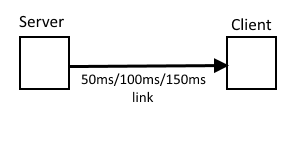
\includegraphics[scale=0.7]{images/topology}
\centering
\caption{Simulated mininet network used for testing: data flowing from a server to a client over a link with one of three defined latencies}
\label{topology}
\end{figure}

Each test was performed using a simulated network on mininet, consisting of a server node connected to a client node over a single link with a specifically defined latency (figure \ref{topology}). This link latency was varied between 50ms, 100ms, and 150ms, and loss rates of 0\%, 0.01\%, 0.1\%, and 1\% were introduced for tests on each latency. Each test ran for 300 seconds with client and server both operating at a framerate of 60 fps; an I-frame was sent every 10th frame, consisting of 4 QUIC packets to represent the fact that I-frames are too large to be sent as a single QUIC payload.


Tests for guaranteed reliability used the \texttt{ngtcp2} QUIC stack with standard retransmission behaviours, while tests for partial reliability used the QUICsilver implementation with partial reliability behaviours described above.

\subsection{Differences in Stack Latency}

Stack latencies remain consistently within 15ms of the path latency in QUICsilver for all loss rates (figure \ref{stack-par}), but have slightly more variance than stack latencies in the guaranteed reliability implementation in equivalent conditions. This is due to the extra checks which are performed by the server after sending a packet: each item in the retransmission buffer for the relevant stream is checked to see if it has become stale and needs to be removed.


When loss is introduced on the link, the guaranteed reliability implementation begins to show an increase in the number of higher stack latencies (figure \ref{stack-rel}). QUIC determines a packet is lost when it receives an acknowledgement for a higher packet number; this requires a minimum of the time taken to send the packet over the link, plus a multiple of the total round trip time depending on how many times the packet in question was lost in transit. This causes the latency data to gather in bands: the latencies of lost packets will be multiples of the total round-trip time on the link. In contrast, QUICsilver maintains similar performance all rates of loss; this is due to the server removing packets which will not be useful to the client upon arrival from its retransmit buffer without receiving an acknowledgement.

\subsection{Differences in Application Latency}

QUICsilver achieves consistently lower application latencies for all link latencies compared to standard QUIC with guaranteed reliability (figure \ref{app-par}). Application latencies for partially reliable QUIC have a greater range than stack latencies due to the frame buffer: if there is a gap in received packets, the stack will wait for the missing packet; if the packet doesn't arrive before its predicted playback deadline expires, the read offsets for the stream are advanced and a sequence of video frames with contiguous RTP timestamps is passed to the application (this may only be a single frame). This buffer was intended to be set as 4 frames, corresponding to an additional latency of 66ms at a 60fps playback rate, but was incorrectly set at a single frame during the 50ms and 100ms tests. A single frame at 60fps is equivalent to 16.7ms; this is added to application latency in the event of loss, with decreasing latencies following as subsequent blocks of received frames are passed to the application. In the case of 150ms tests, the buffer limit was set to the intended 4 frames; application latencies can be seen in bands at multiples of 16.7ms to around a maximum of 66.6ms greater than the link latency as a result.


The distinctive wide band present in all instances of QUICsilver tests is due to I-frames being sent as 4 QUIC packets without a 16.7ms delay between them; four packets must be delivered to the application within the same call, but iterating through the reorder buffer and removing relevant items takes time to execute.


The bands in the standard QUIC application latencies are caused by video frames being sent by the server at 16.7ms intervals; the latency of each frame is increased by a multiple of this until the missing packet is received at the client, even though all of these frames are delivered to the application within the same function call. The occasional spikes in 1\% loss test are caused by a packet being lost twice; these occur at twice the round-trip time, plus two frame playback times at 60fps, beyond the initial link latency.


This head-of-line blocking behaviour associated with guaranteed reliability does not affect 0\% loss links, where standard QUIC achieves consistently lower application latencies than QUICsilver, and has minimal impact on average application latency in 0.01\% loss links. However, for 0.1\% and 1\% loss scenarios, QUICsilver achieves consistently lower application latencies: the latencies for fully reliable QUIC in these circumstances are frequently a round-trip time higher than the link latency, compared to a maximum of 66.6ms when a 4-frame buffer is set.

\clearpage

\begin{figure}
 \centering
 \subfloat[QUICsilver, 50ms]{
   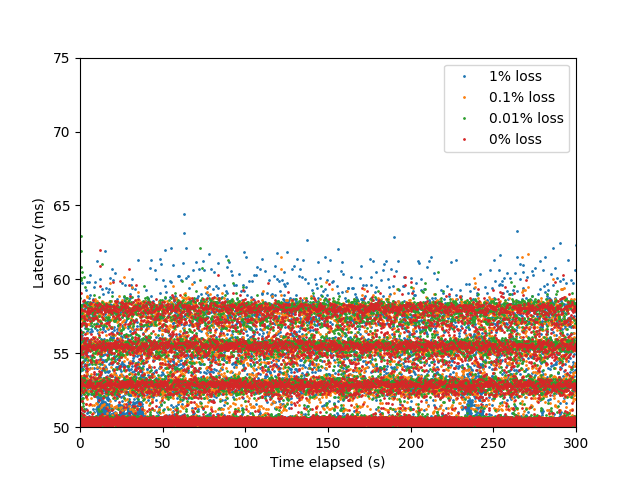
\includegraphics[scale=0.5]{images/graphics-partial/50ms-stack-latencies-combined-PARTIAL.png}
   \label{stack-par-50}
 }
 \\
 \subfloat[QUICsilver, 100ms]{
   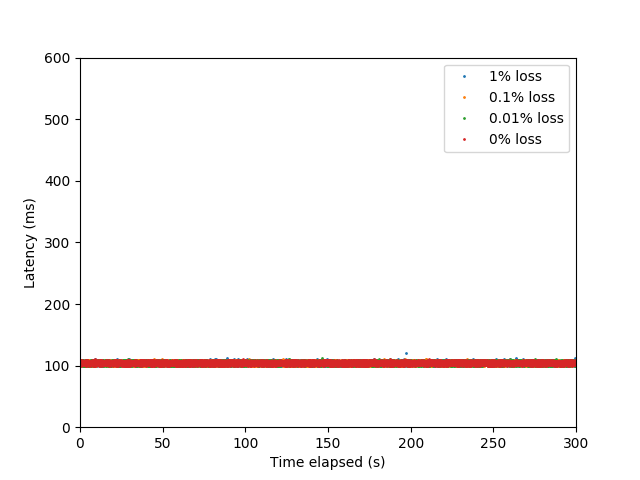
\includegraphics[scale=0.5]{images/graphics-partial/100ms-stack-latencies-combined-PARTIAL.png}
   \label{stack-par-100}
 }
 \\
 \centering
 \subfloat[QUICsilver, 150ms]{
   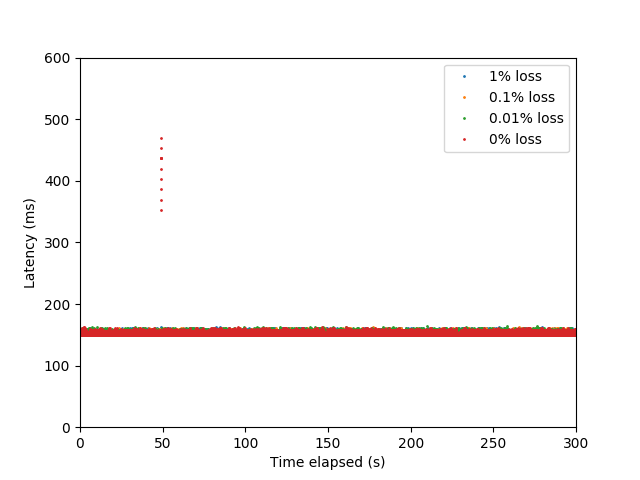
\includegraphics[scale=0.5]{images/graphics-partial/150ms-stack-latencies-combined-PARTIAL.png}
   \label{stack-par-150}
 }
 \caption{Latency between server and client stack (QUICsilver, partial reliability)}
 \label{stack-par}
\end{figure}

\begin{figure}
 \centering
 \subfloat[Standard QUIC, , 50ms]{
   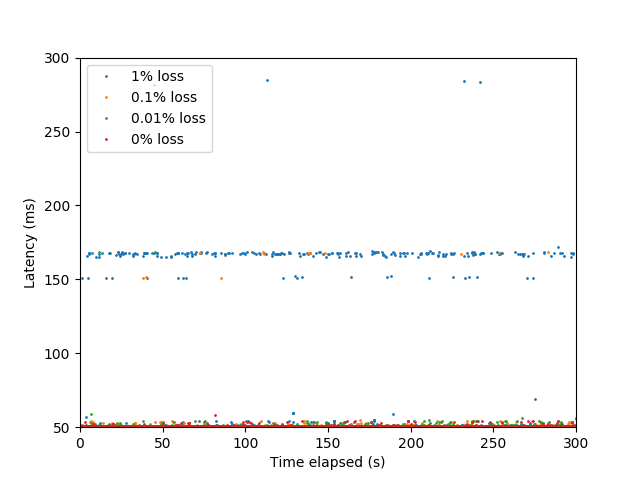
\includegraphics[scale=0.5]{images/graphics-reliable/50ms-stack-latencies-combined-reliable.png}
   \label{stack-rel-50}
 }
 \\
 \subfloat[Standard QUIC, , 100ms]{
   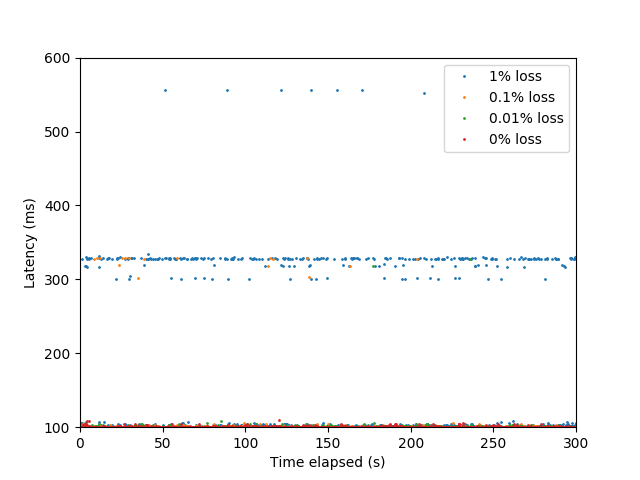
\includegraphics[scale=0.5]{images/graphics-reliable/100ms-stack-latencies-combined-reliable.png}
   \label{stack-rel-100}
 }
 \\
 \centering
 \subfloat[Standard QUIC,  150ms]{
   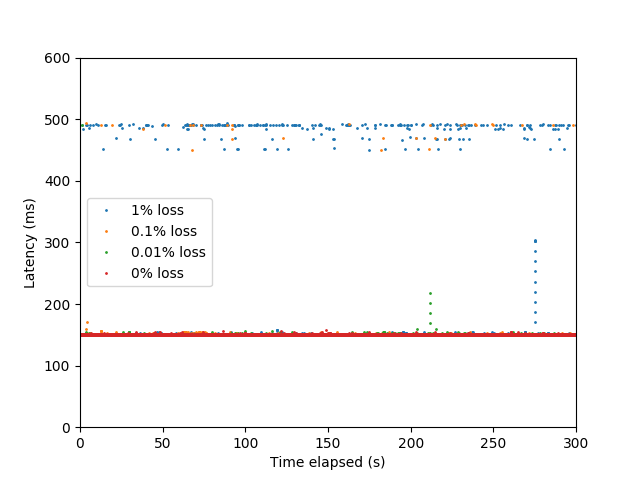
\includegraphics[scale=0.5]{images/graphics-reliable/150ms-stack-latencies-combined-reliable.png}
   \label{stack-rel-150}
 }
 \caption{Latency between server and client stack (standard QUIC, guaranteed reliability)}
 \label{stack-rel}
\end{figure}

\clearpage


\begin{figure}
 \centering
 \subfloat[QUICsilver, 50ms]{
   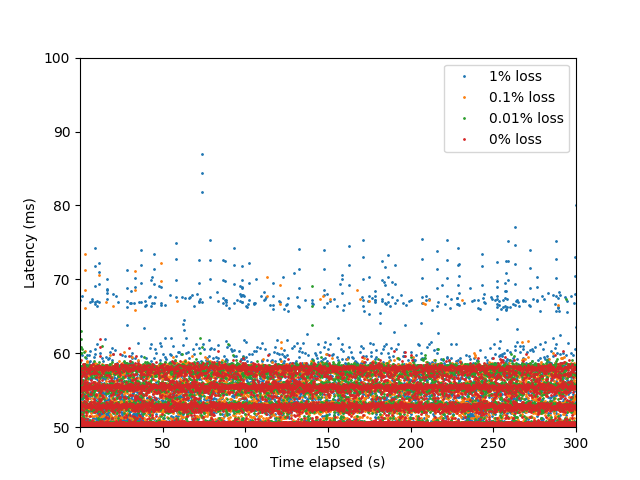
\includegraphics[scale=0.5]{images/graphics-partial/50ms-app-latencies-combined-PARTIAL.png}
   \label{app-par-50}
 }
 \\
 \subfloat[QUICsilver, 100ms]{
   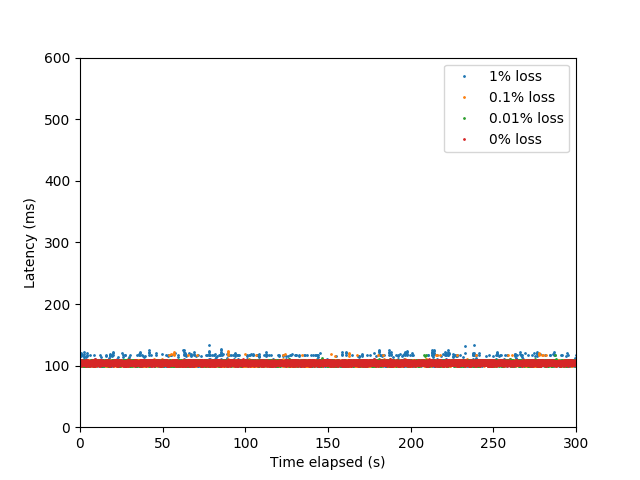
\includegraphics[scale=0.5]{images/graphics-partial/100ms-app-latencies-combined-PARTIAL.png}
   \label{app-par-100}
 }
 \\
 \centering
 \subfloat[QUICsilver, 150ms]{
   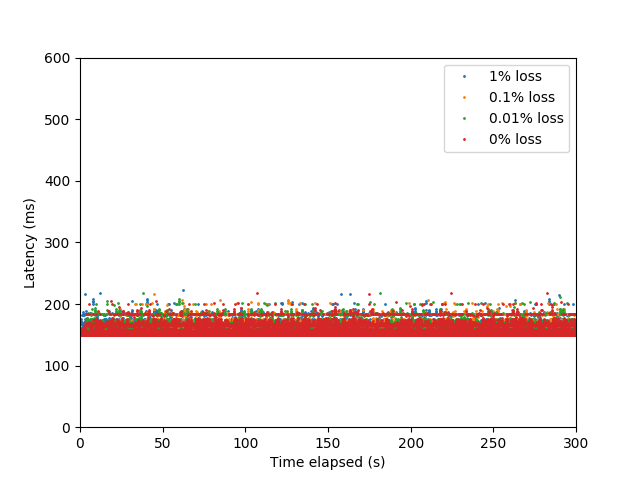
\includegraphics[scale=0.5]{images/graphics-partial/150ms-app-latencies-combined-PARTIAL.png}
   \label{app-par-150}
 }
 \caption{Latency between server and client application (QUICsilver, partial reliability)}
 \label{app-par}
\end{figure}

\begin{figure}
 \centering
 \subfloat[Standard QUIC, 50ms]{
   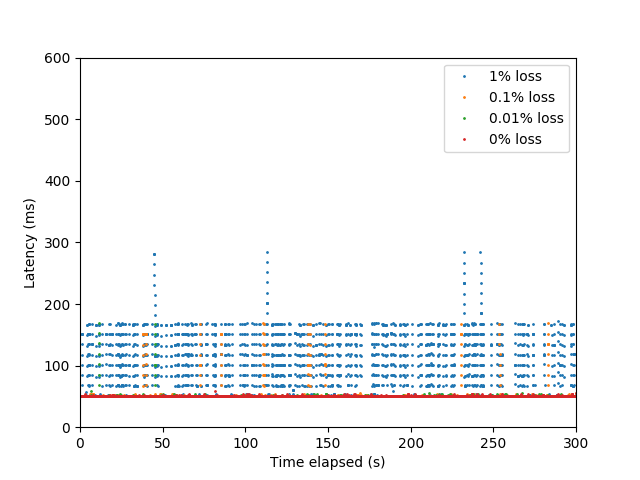
\includegraphics[scale=0.5]{images/graphics-reliable/50ms-app-latencies-combined-reliable.png}
   \label{app-rel-50}
 }
 \\
 \subfloat[Standard QUIC, 100ms]{
   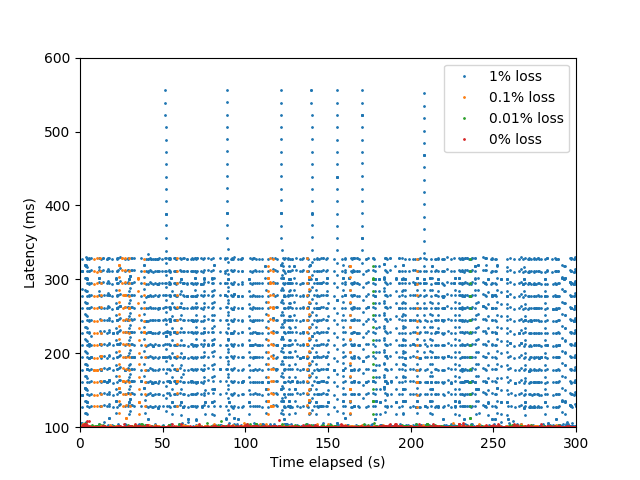
\includegraphics[scale=0.5]{images/graphics-reliable/100ms-app-latencies-combined-reliable.png}
   \label{app-rel-100}
 }
 \\
 \centering
 \subfloat[Standard QUIC, 150ms]{
   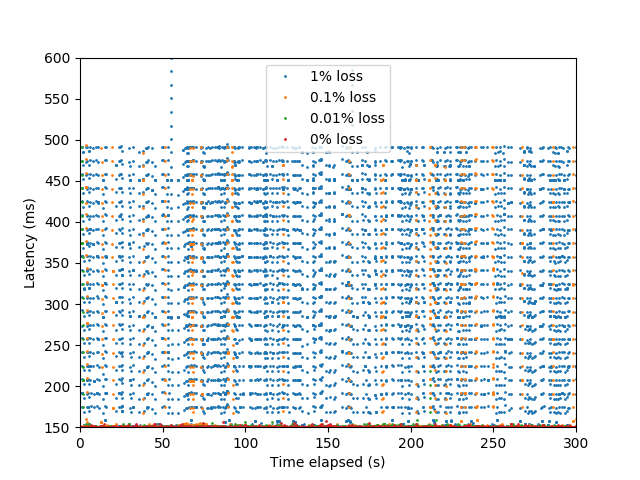
\includegraphics[scale=0.5]{images/graphics-reliable/150ms-app-latencies-combined-reliable.png}
   \label{app-rel-150}
 }
 \caption{Latency between server and client application (standard QUIC, guaranteed reliability)}
 \label{app-rel}
\end{figure}




% The details

% Describe results carefully:
%  - clearly state assumptions
%  - give enough information to allow the reader to recreate the results
%  - ensure results are representative; statistically meaningful, etc.
%  - don't overstate results
%  - equally, don't understate them: consider the broader implications


\clearpage
\subsection{Differences in Playback Time}

If a packet has been lost in transit, the head-of-line blocking behaviours within standard QUIC will delay delivering all subsequent data until this missing packet has been received. If there is no video data held in the application to play during this delay (i.e. buffered data), the video will appear to stall. The exact delay caused by a packet lost once is proportional to the path latency: figure \ref{single-50} shows a delay of 100ms, the round trip time of a 50ms link. Figure {single-100} shows a delay of 216ms on a 100ms link, equivalent to a round trip time plus one frame playback time; this extra 16ms is likely due to these measurements being obtained in terms of RTP playback timestamps, with a granularity of 16ms per increment at 60fps. The delay for a loss on a 150ms link shown in figure \ref{single-150} is 333ms, equivalent to one round-trip time plus one frame playback time.


\begin{figure}
 \centering
 \subfloat[Single instance playback delay, 50ms]{
   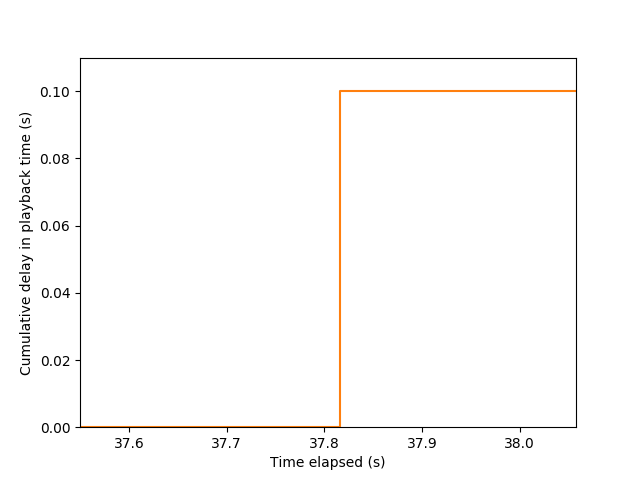
\includegraphics[scale=0.5]{images/offsets-single.png}
   \label{single-50}
 }
 \\
 \subfloat[Single instance playback delay, 100ms]{
   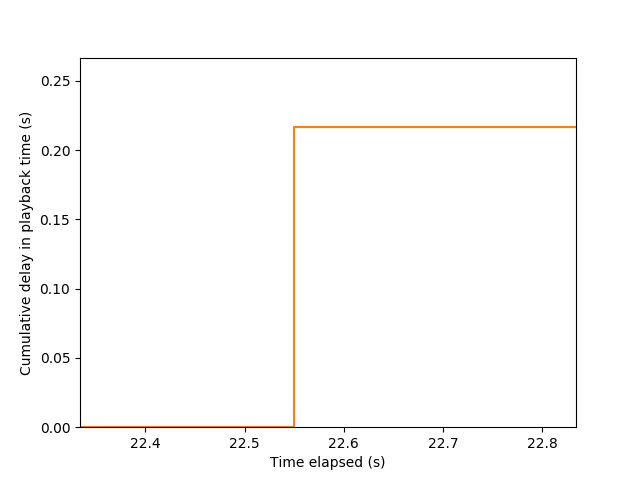
\includegraphics[scale=0.5]{images/offsets-single-100ms.png}
   \label{single-100}
 }
 \\
 \centering
 \subfloat[Single instance playback delay, 150ms]{
   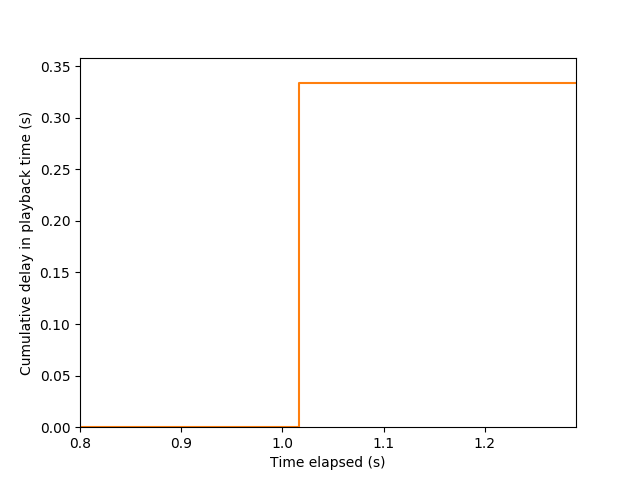
\includegraphics[scale=0.5]{images/offsets-single-150ms.png}
   \label{single-150}
 }
 \caption{Increase in cumulative playback delay as a result of a single lost packet on various links (standard QUIC, guaranteed reliability)}
 \label{single-rel}
\end{figure}


As the rate of loss on a link increases, the number of stalls also increases. Table \ref{reliable-stalls} shows the number of stalls which occured in the 100ms tests; naturally, the number of stalls between all latencies remain similar for each loss rate, but the difference between intended playback time and actual playback time for each subsequent video frame becomes larger at higher latencies (table \ref{relative-offset-table}). The graphs shown in figure \ref{playback-rel} illustrate the magnitude of these differences.

\begin{table}[h!]
\centering
\label{stalls-data-rel}
\begin{center}
%\begin{tabular}{|p{5cm}|l|p{8.5cm}|}
\begin{tabular}{|p{2cm}|p{2cm}|p{2cm}|}
\hline
Loss Rate & Stalls & Frames Played\\ \hline
0\% & 0 & 100.0\% \\ \hline
0.01\%  & 2 & 100.0\% \\ \hline
0.1\%  & 12 & 100.0\% \\ \hline
1\%  & 198 & 100.0\% \\ \hline

\end{tabular}
\caption{Number of stalls and percentage of frames played for standard QUIC, 100ms}
\label{reliable-stalls}
\end{center}
\end{table}

\begin{figure}
 \centering
 \subfloat[Playback offsets, 50ms]{
   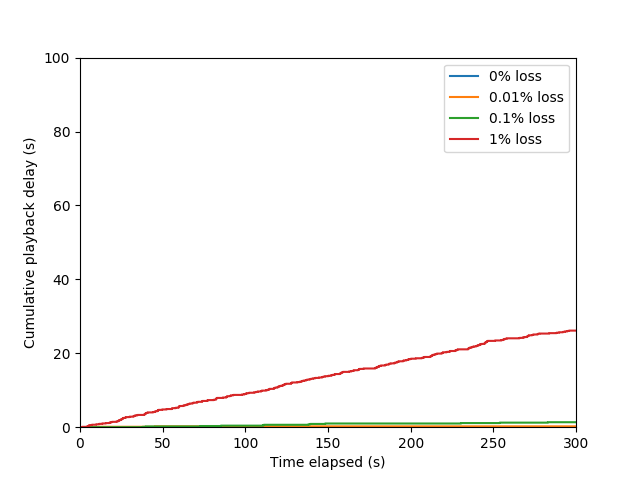
\includegraphics[scale=0.5]{images/graphics-reliable/50ms-offsets-combined-reliable.png}
   \label{playback-rel-50}
 }
 \\
 \subfloat[Playback offsets, 100ms]{
   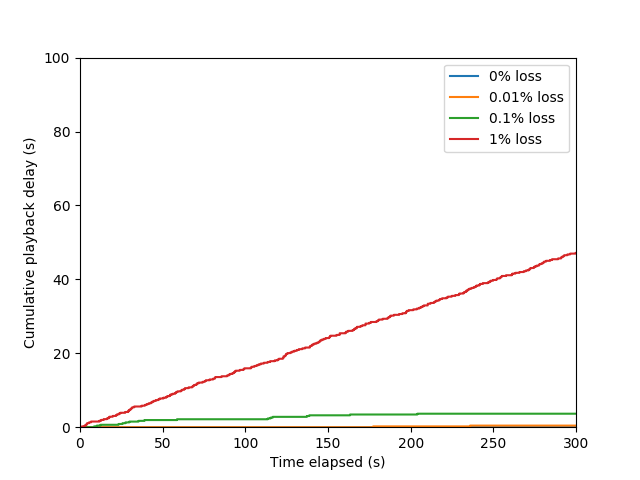
\includegraphics[scale=0.5]{images/graphics-reliable/100ms-offsets-combined-reliable.png}
   \label{playback-rel-100}
 }
 \\
 \centering
 \subfloat[Playback offsets, 150ms]{
   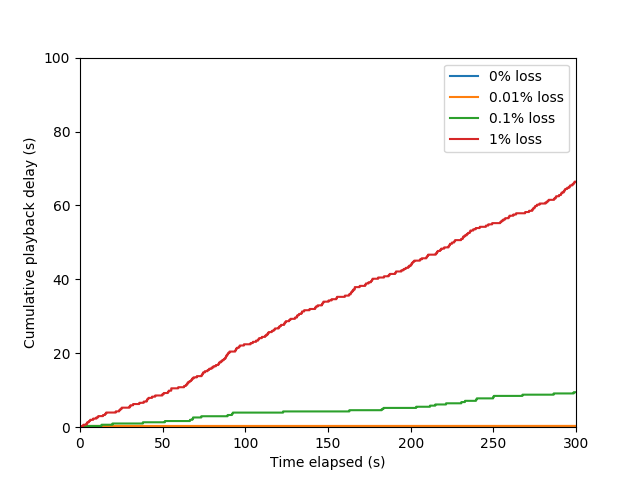
\includegraphics[scale=0.5]{images/graphics-reliable/150ms-offsets-combined-reliable.png}
   \label{playback-rel-150}
 }
 \caption{Differences between when a frame is played out compared to the intended playback time (standard QUIC, guaranteed reliability)}
 \label{playback-rel}
\end{figure}

\begin{figure}
 \centering
 \subfloat[Playback times, 50ms]{
   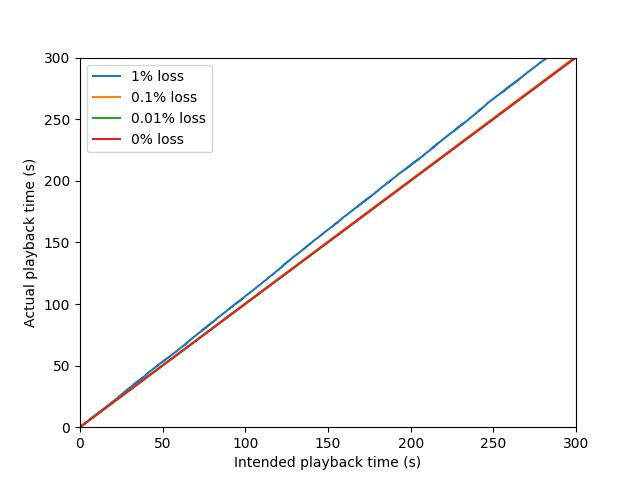
\includegraphics[scale=0.5]{images/graphics-reliable/50ms-relative-offsets-combined-reliable.png}
   \label{playback-offsets-rel-50}
 }
 \\
 \subfloat[Playback times, 100ms]{
   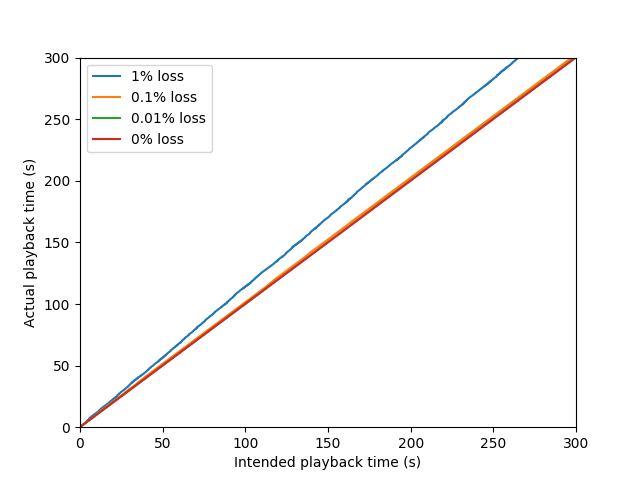
\includegraphics[scale=0.5]{images/graphics-reliable/100ms-relative-offsets-combined-reliable.png}
   \label{playback-offsets-rel-100}
 }
 \\
 \centering
 \subfloat[Playback times, 150ms]{
   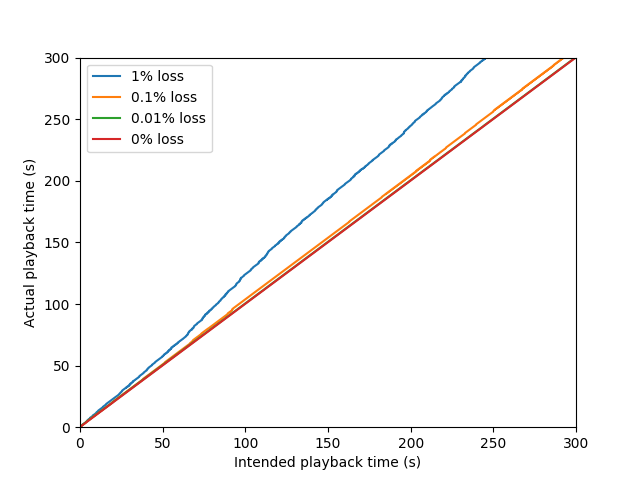
\includegraphics[scale=0.5]{images/graphics-reliable/150ms-relative-offsets-combined-reliable.png}
   \label{playback-offsets-rel-150}
 }
 \caption{Differences between when a frame is played out compared to when the frame was sent (standard QUIC, guaranteed reliability)}
 \label{playback-offsets-rel}
\end{figure}

\begin{table}[h!]
\centering
\label{stalls-data-rel}
\begin{center}
%\begin{tabular}{|p{5cm}|l|p{8.5cm}|}
\begin{tabular}{|p{1.5cm}|p{1.5cm}|p{2cm}|p{2cm}|}
\hline
Loss Rate & Latency (ms) & Discrepancy (s) & Total latency (s)\\ \hline
0.01\%  & 50 & 0.2 & 50.2 \\ \hline
0.1\%  & 50 & 1.2 & 51.2 \\ \hline
1\%  & 50 & 19.8 & 69.8 \\ \hline
0.01\%  & 100 & 0.43 & 100.43 \\ \hline
0.1\%  & 100 & 2.6 & 102.6 \\ \hline
1\%  & 100 & 42.8 & 142.8 \\ \hline
0.01\%  & 150 & 0.66 & 150.66 \\ \hline
0.1\%  & 150 & 4.0 & 154.0 \\ \hline
1\%  & 150 & 66.0 & 216.0 \\ \hline

\end{tabular}
\caption{Playback discrepancy and total latency for a live-recorded frame to be played by the client application at the end of each test run for each loss rate and latency for standard QUIC}
\label{relative-offset-table}
\end{center}
\end{table}

Table \ref{relative-offset-table} shows the cumulative discrepancy between intended playback time and actual playback time, as well as the delay between a live-recorded frame being sent and being played by the client application by the end of a 300 second test run. The increase in this delay over time is illustrated in figure \ref{playback-offsets-rel}.


Although 100\% of the video frames in the media content being sent are delivered to the client application with guaranteed reliability behaviours, there is an increasing latency between sending a frame and playing it at the client; the longer an application is running, the greater this playback discrepancy becomes. The path latencies in these tests were constant, but path latencies `in the wild' are variable, and occasionally subject to spikes if a link is congested. The total playback discrepancy suffered by an application would sharply increase as a result of these spikes; a return to lower latencies afterwards would not reduce it.


It should also be noted that this discrepancy is applied to packets which have not been lost in transit: lost packets are subject to even higher latencies, and are increased by multiples of the round-trip time depending on the number of times they are lost. As shown in figure \ref{app-rel}, packets which have been received before a missing packet but have a higher packet number also suffer from increased application latency. International Telecommunication Recommendation G.114 recommends no more than 150ms latency ``mouth-to-ear'' for audio communications \cite{ITU-REC}; the path latency must be even smaller than this to allow for time to capture live audio and video and to perform codec processing. Figure \ref{app-rel} shows that fully reliable QUIC stays within this limit at 0\% and 0.01\% loss for 50ms and 100ms links, but it often exceeds even the ``mouth-to-ear'' limit at 0.1\% and 1\% loss for all links; 0\% and 0.01\% loss flows on a 150ms link cannot satisfy the recommended latency requirement due to the link latency.


In the case of video streaming, content buffering can be used to disguise stalls. For example, if a user wanted to stream a 1 hour, pre-recorded video, the client might buffer a given amount of content before starting playback. Given that an I-frame is sent every 10th frame as 4 QUIC packets, 216,000 video frames will be sent using 280,800 QUIC packets in total: 28 stalls can be expected to occur at 0.01\% loss, 281 stalls at 0.1\% loss, and 2808 stalls at 1\% loss. At a cumulative latency increase of 100ms per lost packet on a 50ms link, a buffer of 200 seconds should completely conceal stalls for 0.01\% and 0.1\% loss rates, and will conceal stalls at 1\% until 2564 seconds (around 43 minutes) into playback. For a 100ms link with a 216ms latency increase, a buffer of 200 seconds should completely conceal stalls for 0.01\% and 0.1\% loss rates, and will conceal stalls until 1183 seconds (around 20 minutes) into playback. A 400 second buffer should conceal all stalls. However, buffering is not a feasible strategy for reducing the number of stalls in real-time media delivery: live-generated content cannot be buffered in advance, and buffering does not reduce the cumulative playback delay created as a result of stalls in fully reliable QUIC.


QUICsilver experiences no stalls due to incrementing stream read offsets in response to playback deadlines: if there is a gap in the data received on a given stream and there is data approaching its playback deadline held in the reorder buffer, the modified implementation will skip ahead to the live data and will not wait for the preceding gap to be filled. This allows the client to play received content without additional delays caused by head-of-line blocking. The percentage of `useful frames' in table \ref{par-playback-stats} is calculated as the number of complete I-frames and P-frames with an associated complete I-frame, compared to the total number of unique frames sent by the server; incomplete I-frames and their subsequent P-frames are not useful for playback.

\begin{table}[h!]
\centering
\label{stalls-data-par}
\begin{center}
%\begin{tabular}{|p{5cm}|l|p{8.5cm}|}
\begin{tabular}{|p{2cm}|p{2cm}|p{2cm}|}
\hline
Loss Rate & Stalls & Useful frames\\ \hline
0\% & 0 & 100.0\% \\ \hline
0.01\%  & 0 & 100.0\% \\ \hline
0.1\%  & 0 & 99.644\% \\ \hline
1\%  & 0 & 95.472\% \\ \hline

\end{tabular}
\caption{Number of stalls and percentage of useful frames played for QUICsilver}
\label{par-playback-stats}
\end{center}
\end{table}

\begin{figure}[h]
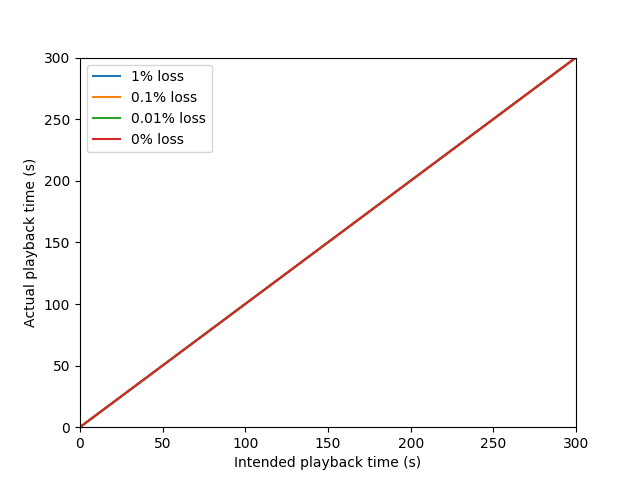
\includegraphics[scale=0.5]{images/graphics-partial/50ms-relative-offsets-combined-PARTIAL.png}
\centering
\caption{Differences between when a frame is played out compared to when the frame was sent (QUICsilver, partial reliability, all loss rates)}
\label{playback-par}
\end{figure}

Fewer frames are played back at the client, which will result in occasional glitches in playback. Given that 1 in every 10 frames sent is an I-frame consisting of 4 QUIC packets, there is a 70\% chance that a dropped packet contains a P-frame; at a playback rate of 60fps, this would result in an absence of updated content for 16.7ms. If a dropped packet contains a section of an I-frame, this will affect the subsequent 9 P-frames which are dependent on it; this would result in no the appearance of glitched content for 167ms due to P-frames acting in reference to an incorrect I-frame.


As described in section 3, QUICsilver is capable of performing retransmissions of live I-frames and P-frames, and stale I-frames which are still required for live P-frames. A 4-frame delay adds a maximum of 66.6ms additional latency between the server and the client application, which would create a total maximum of 116.6ms on a 50ms link; this is already relatively high for a real-time application. Removing this delay entirely results in the implementation achieving the lowest possible latency while effectively transmitting P-frames unreliably and retransmitting I-frames once at most.


Whether a stale I-frame can be retransmitted to enable the playback of future P-frames depends on the path latency: if an I-frame is sent once every 10 frames, there is a a space of 150ms between I-frames being played back. Given that a retransmission takes one round-trip time in total, an I-frame fragment would enable the 9th subsequent P-frame if it was sent over a 66.6ms latency link; lower latencies would allow a larger number of associated P-frames to be played successfully, while any latency above this would not perform any retransmissions and would function as an unreliable transport. Sending I-frames less frequently would allow a larger window for I-frame fragments to be retransmitted, but the amount of glitched playback would increase in proportion with the link latency; the longer an application has to wait for a complete I-frame, the more P-frames are played in reference to the incorrect I-frame.


For a test run of 300 seconds, 18,000 video frames are sent. On average 180 of these are dropped in the worst-case 1\% loss scenario; if 30\% of these are I-frames and 70\% are P-frames, 11.01 seconds of playback in total are subject to glitches across all latencies. This is higher than the total playback offset in a 50ms connection subject to 1\% loss for standard QUIC (table \ref{relative-offset-table}), but the crucial difference between these two outcomes is that the content received after a loss in QUICsilver is played without any cumulative delay (figure \ref{playback-par}): some playback quality is sacrificed for maintaining a consistent low latency to allow for the level of responsiveness required by real-time applications.


An application using guaranteed reliability could discard stale frames and continue playback from the frame with the closest RTP timestamp to the current playback deadline to reduce this cumulative delay, but it would play fewer frames than the partially reliable implementation: the minimum and maximum absences of correctly updated content for partially reliable QUIC for all link latencies are 16.7ms and 167ms respectively, while delays in the datasets gathered for fully reliable QUIC range between 100ms and 333ms, depending on the link latency. This shows that QUICsilver results in improved throughput of useful data compared to attempting to optimise applications on top of standard QUIC for real-time behaviour.

%==================================================================================================
%\section{Related Work}

% This should come near the end, and focussing on discussing how your work
% relates to that of others. Any relevant related work should have been
% cited already, so this is not a list of related work, it's a discussion
% of how that work relates.
%
% Why not put related work after the introduction? 1) because describing
% alternative approaches gets between the reader and your idea; and 2)
% because the reader knows nothing about the problem yet, so your
% (carefully trimmed) description of various technical trade-offs is
% absolutely incomprehensible.
% 
% When writing the related work:
%  - Give credit to others where it's due; this doesn't diminish the
%    credit you get from your paper. 
%  - Acknowledge weaknesses in your approach.
%  - Ensure related work is accurate and up-to-date



%==================================================================================================
%==================================================================================================
\section{Future Work}

\subsection{Congestion Control}
Removing an item from the retransmission buffer in the \texttt{ngtcp2} implementation of QUIC is complex. The function call used to receive an acknowledgement contains numerous updates to congestion control statistics; simply attempting to remove the item from the retransmit buffer by freeing the associated memory causes a range of errors due to failed \texttt{assert} checks elsewhere in the stack. As a result, falsified acknowledgements were created at the server to remove stale entries which had not received an acknowledgement from the client. This is problematic in that it causes the client to believe there is no congestion on the network, and this QUIC flow becomes overly aggressive compared to other flows sharing the link as a result. This did not cause problems with testing on the simple one-to-one topology with a known round-trip time and no co-existing flows described in section 4, but the congestion control statistics must be more carefully adjusted in future iterations to allow real-time QUIC flows to be fair to other traffic on shared links.


\subsection{Improved I-frame Handling}
QUIC packets containing fragments of I-frames which will not arrive in time to be played back themselves, but are required for live P-frames are retransmitted by the server. An implementation of real-time QUIC which immediately passes data to the application upon arrival would deliver these `stale' fragments to the application, however, the implementation of partial reliability which delivers video frames in order does not; the stream read offsets at the client are incremented upon the delivery of live data and the detection of stale data, so these I-frame fragments are never passed to the application.


Future refinements of QUICsilver would include mechanisms to allow the client to determine if an incoming packet contains an I-frame based on its associated RTP timestamp, and introducing additional read offsets within a stream to allow required stale I-frames to be read without also reading stale P-frame data in the process. This would allow complete frames to be delivered in-order to the application, while continuing to drop stale P-frames and stale I-frames with no live dependencies to minimise latency. I-frame payloads would also need to be read as a complete block to allow delivery to the application as a complete frame, as opposed to the current method of being delivered as several separate reads.


\subsection{Multiple Streams}
Real-time QUIC will allow multimedia application developers to use multiplexed streams to deliver data to an application concurrently, but this significantly increases the difficulty in developing these applications: the content received from each stream needs to be co-ordinated in order to be used by the application correctly. The tests in this paper were performed using a single stream; further experiments will focus on how to co-ordinate multiplexed streams to optimise the quality of video playback.

%==================================================================================================
\section{Conclusions}

\subsection{Placement of Complexity}
Passing QUIC payloads (i.e. RTP packets) to the application as soon as they arrive avoids adding even more complexity to an already extensive transport protocol, but it requires application developers to implement mechanisms to reorder incoming frames, assemble I-frames, and deal with frames which are corrupted, incomplete, or missing dependencies; the transport protocol effectively becomes RTP with selective retransmissions. This allows developers flexibility in exactly how a given application should behave while improving the amount of useful data received, but it increases both the entry barrier to creating real-time multimedia applications and the difficulty in maintaining them.


Delivering complete video frames in-order while allowing gaps, as the implementation of real-time QUIC in this project aims to do, removes the responsibility of frame reordering and reconstruction from application developers, but increases the complexity of QUIC while also restricting the applications which can be developed: novel applications, such as multiplayer gaming over QUIC, may require many different types of messages other than I-frames and P-frames. Awareness of these messages would need to be added within the QUIC protocol in order for a receiver to be able to parse stream information as a complete message, and for the sender to be able to establish more complex dependencies and retransmission behaviours; for example, an important message such as a character receiving an item should be transmitted with guaranteed reliability and only removed from the retransmission buffer with a client-sent ACK, while movement would use partial reliability and deadline-based removal in a similar manner to P-frames. This is simply not feasible given the wide range of behaviours and transmittable information that real-time applications could have.


\subsection{Partial Reliability for Other Real-Time Applcations}
The development of video-based real-time applications which rely on a limited number of message types (I-frames and P-frames) can be simplified by making QUIC aware of how to parse these messages and pass them to the application as complete frames in sequential order; this project has been successful in achieving improved real-time video playback performance using this approach. However, the increasing popularity of real-time applications with variable information and behaviour, such as augmented reality, virtual reality, and multiplayer gaming, suggests that passing data to the application as soon as it arrives is the better approach to take for a generalised real-time implementation of QUIC. This prevents ossification in terms of which applications which can use real-time QUIC and also avoids adding an unrealistic level of complexity to QUIC implementations. Creating a new partially reliable QUIC stream type for use alongside guaranteed reliability streams would ensure that key information reaches the receiver while allowing low-latency for other content.


\subsection{Utility of QUICsilver}
%Adjustments to the rate at which I-frames are sent would allow I-frame retransmissions to allow subsequent P-frames to be played correctly; at the current rate of 1 in 10 frames, QUICsilver effectively performs as an unreliable transport at path latencies above 66.6ms.

Standard QUIC is more suited for high-quality video streaming than QUICsilver: pre-existing content can be buffered in advance to mask stalls, and 100\% of frames are played without glitches. Buffering pre-existing content could also be performed with QUICsilver, but the stack and application latencies would increase due to performing liveness checks on many items which would be stored in the retransmit and reorder buffers at the client and server respectively; this is wasted time given that these checks to prevent stalls are not necessary when stalls are already being masked by buffered content.

However, QUICsilver provides far better performance for applications which transmit data live and require timely responses to user input than standard QUIC. It achieves this by adjusting its stream read offsets and removing items from its retransmit buffers in response to playback deadlines, yielding consistently lower application latencies at all link latencies and loss levels. This results in intermittent glitches in video playback, but over 95\% of unique frames sent by the server are played back without glitches even in 1\% loss environments.

ClipStream, the alternate partially reliable QUIC implementation discussed in section 3 \cite{Palmer2018}, encounters stalls very rarely due to I-frames being transmitted reliably. QUICsilver, however, eliminates stalls completely though use of deadline awareness, ensuring that zero cumulative playback latency occurs at any loss rate and therefore preventing extended sessions of real-time media applications from suffering an increasing cumulative playback delay. This consistent, predictable low-latency performance makes QUICsilver a promising option for running responsive, real-time applications over QUIC.

%more accurate measuring of useful frames if data delivered in-order to application as complete frame - incomplete I-frame would still pose problems even if data was immediately passed to application from stack

%==================================================================================================
\section{Acknowledgements}

I would like to thank my advisor, Dr Colin Perkins, for introducing me to the hydra that is the inner workings of the modern Internet and for providing advice on how to make contributions to an exciting new transport protocol. I would also like to thank the many friends who helped keep morale high through every new segmentation fault.

\bibliographystyle{abbrv}
\bibliography{example}


\end{document}
